After building up intuition on the biological features of a Drosophila embryo and a model capable of (crudely) mimicking it, we can now begin probing our model for interesting phenomena.\\
\todo{Give me all the questions again}\\
We know nature has a handful symmetry breaks which are kept enacted through self-[interacting] feedback loops. Having added a minimal number of these, we would simply like to see whether vivo-like gastrulation can emerge. Focusing not just the final structures; but also the individual events leading up to it. \todo{Flet\textit{ No explicit timing (BC, IC)} ind}\\
 
Once we have assessed the phenomenological validity of our model, we will look onward for intriguing natural phenomena to study. Given our full embryo model from [individual constituents], simulating separate events, we will be looking into the interplay between these [constituents] and events. This will be compared to known examples of domain-interaction in vivo.\reph\\


On the structure: In the following sections we will go through the similarities between simulation and reality, starting from simple visual comparisons, ending in detailed quantifications. We will do these for the different events (A1-A3) and embryo domains. Afterwards, we will be looking at removing different active parts of the simulated embryo, comparing the results to known real-life mutants. This will finally lead us to a purely in-silico analysis of the event-interactions, including a parameter sensitivity analysis and [something more i hope].\\ 

\renewcommand{\contentsname}{Results Section Table of Contents}
 \setcounter{tocdepth}{2}
\localtableofcontents
\renewcommand{\contentsname}{Table of Contents}
 \setcounter{tocdepth}{1} 


\newpage

\section{Qualitative Agreement}
While the Drosophila embryo has been studied for decades, it is only relatively recently that microscopy and computer science has gotten to a point where quantitative analyses of the more than 5000 cells have become feasible. Therefore, like in most of the fields history, we will start with visually examining the morphology of the embryo. 

For all figures in this paper, If nothing else is noted, the run is [define run]. In vivo, the time of invagination of the posterior midgut (\pmg{A3} in the overview) is about 12 minutes after start, the timing of the simulation is defined to align with this event, allowing for direct comparisons in "minutes" across simulated and experimental timelines.\\


We will start out this section with an overview which we compare to imaged embryos to ensure that there is general phenomenological agreement. We will then go through the individual main morphological events (\vf{A1}, \gb{A2} and \pmg{A3} from Figure \ref{fig:big-timeline}) and qualitatively assess the resemblance between the simulated events and real embryos, hopefully providing some preliminary insight into the [simulated] mechanics. Finally, we will make some additional visual annotations to aid in estimating the nature of the tissue movements, which will help facilitating a more intuitive understanding of these developmental changes.

On the following page, we [compare] our best in silico model and corresponding frames from a video by [Stas' group]: \todo{more specific about video, and explain visuals succinctly}
\newpage

\begin{figure}[H]
    \centering
    \vspace*{-1cm}\hspace*{-1cm}\makebox[\textwidth]{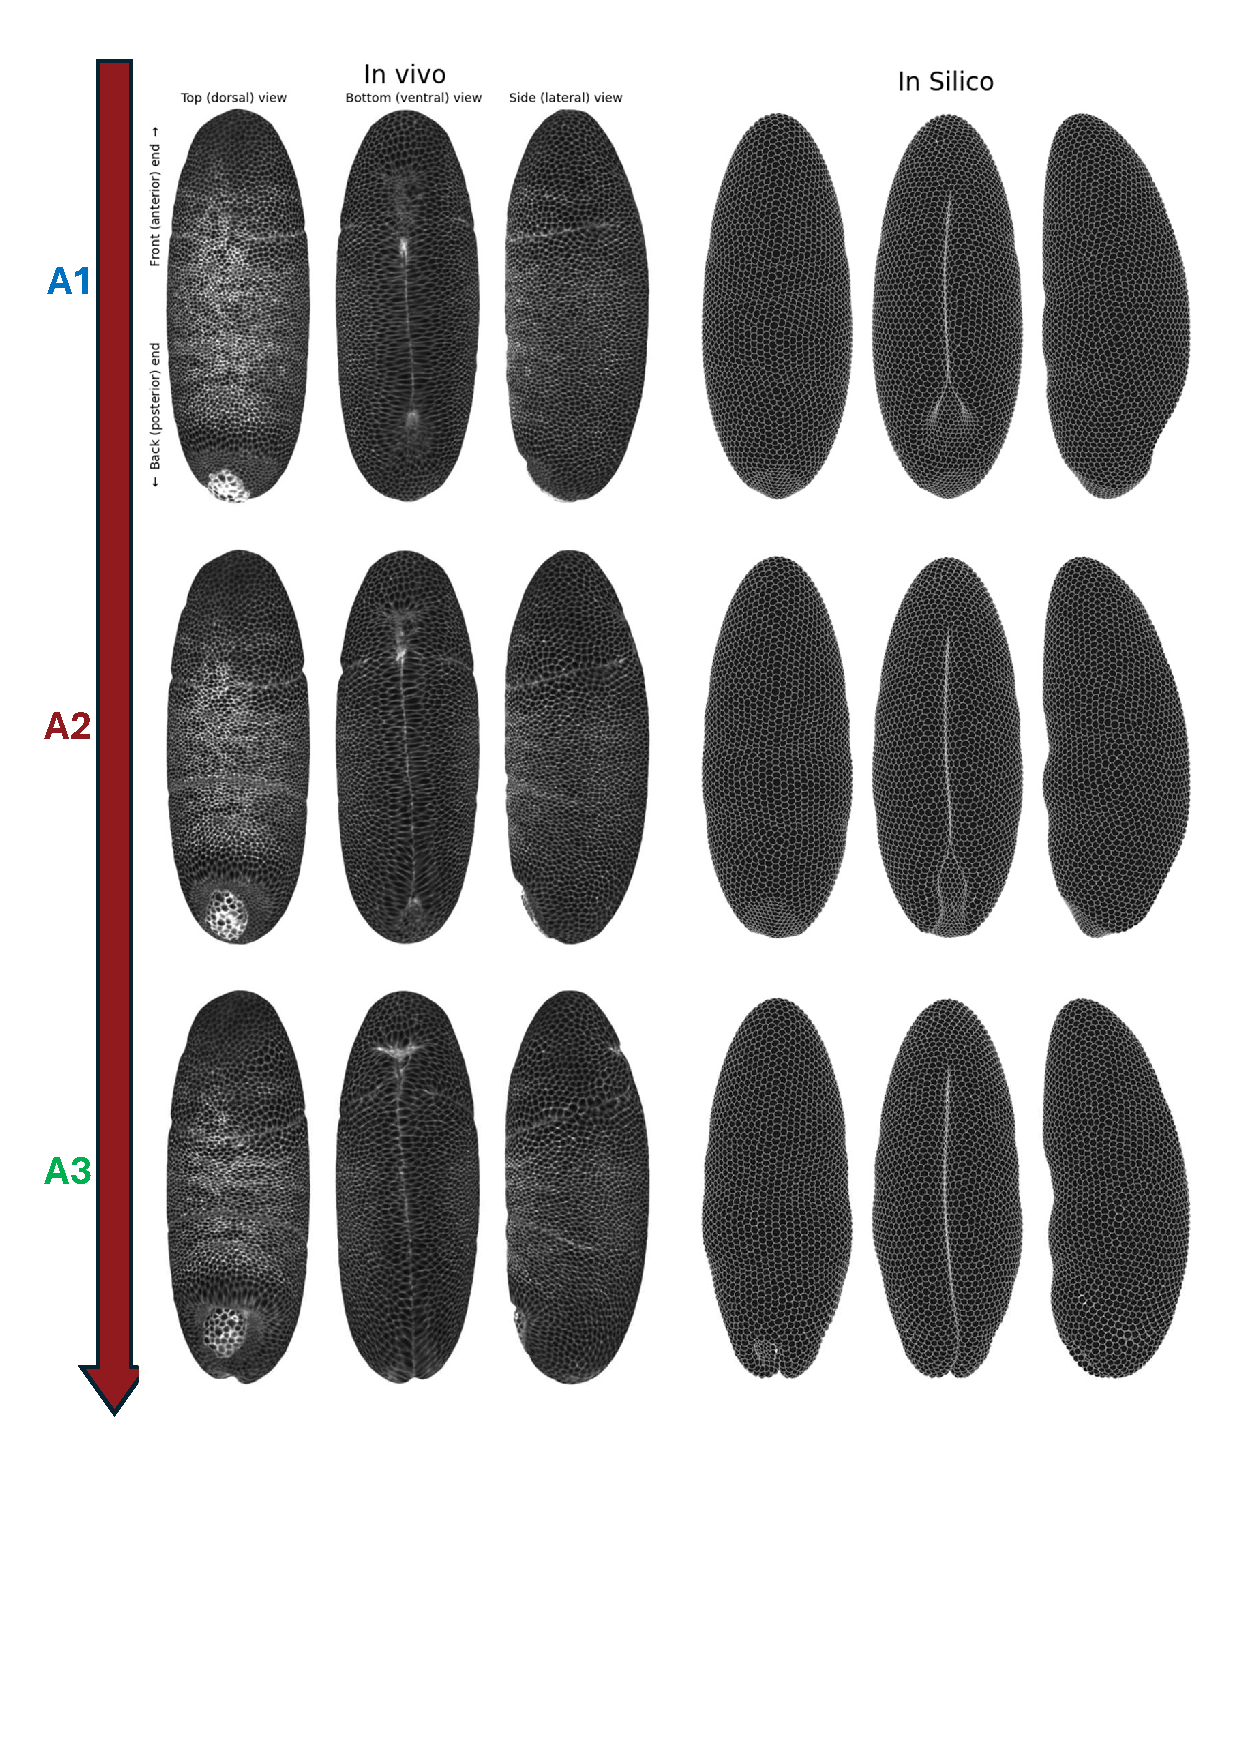
\includegraphics[width=0.85\paperwidth]{chapters/Results/figures/compare_to_vid_timeline_v2.pdf}}
    \caption{Caption on next page}
    \label{fig:big-visual-comparison}
\end{figure}
\newpage
\addtocounter{figure}{-1}
\begin{figure} [t!]
  \caption{(Previous page.) \\A full page visual comparison between three time steps of the simulation and in vivo imaging. 
  Each row consists of a single time-step. For the sake of comparison, the colors have been matched.\\
  \textbf{Left:} In vivo. \textbf{Right:} In silico.\\Within each row, the embryo is show from the top (dorsally), bottom (ventrally) and side (laterally), with the back end (posterior) pointing downwards.}
\end{figure}



It is easy to hide behind numbers and advanced analytical methods, so for completeness sake we have started by presenting a visually unaltered full-scale comparison. Our analyses will soon be more sophisticated, but from a naive inspection, the general dynamics, timing and shape seems to generally have been recapitulated. Given the relatively simple model and few specific alterations, this is already notable! we can see that ... \\ 


To completely understand the agreements between data and simulation we will need to scrutinize the individual pieces using some visual aids. Using the main events (\vf{A1}, \gb{A2}, \pmg{A3}) as starting points, we will go to a higher level of resolution, focusing on individual parts of the embryo, validating the simulation and comparing them to in-vivo imaging when available.


\subsection{Ventral Furrow (\vf{A1})}
The the first sign of movement on the embryo is on the belly where a distinct cleft begins forming. \\
This is called the \vf{ventral furrow} and is the first point of creation for the tubes that will become the gastrointestinal tract.

Closes off in just over three minutes
\textit{A rapid, membrane-dependent pathway directs furrow formation through RalA in the early Drosophila embryo}
As the furrow closes, the internalized cells form a tube with a recognizable light bulb-shape in the cross section. \\
\todo{Add outside-imaging?}\\


Below, in Figure \ref{fig:VFComparison}, a comparison between a cross section of our simulation and in vivo imaging can be seen.

\begin{figure}[H]
    \centering
    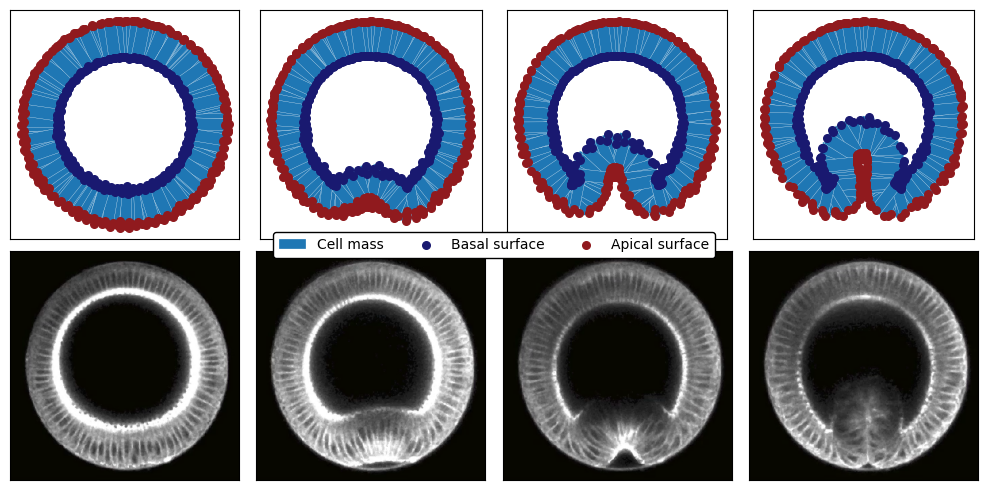
\includegraphics[width=1\linewidth]{chapters/Results/figures/VF_comparison.png}
    \caption{A comparison of simulation and frames from video of live growth. For making it visually more alike, each cell in the simulation is displayed as a rectangle with the longer side aligning with its simulated apical-basal-axis. The blue and red dots are approximations of the inner and outer cell walls. $\textbf{r} + a\textbf{p}$ and $\textbf{r}-a\textbf{p}$ respectively (for position $\textbf{r}$ and AB-vector $\textbf{p}$ and some scale constant \textit{a}).  \\\textbf{Upper row}: Simulation at four different, equally spaced time points. \\\textbf{Lower row}: Multi-photon microscopy of cell walls during ventral furrow formation (Source: \citeAY{conte2012biomechanical}). \\}
    \label{fig:VFComparison}
\end{figure}

\begin{figure}[H]
    \centering
    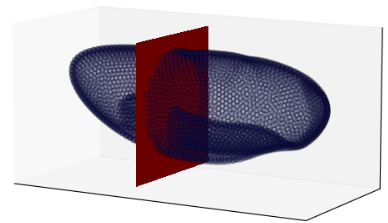
\includegraphics[width=0.65\linewidth]{chapters/Results/figures/planecut2.png}
    \caption{The cutting plane used in Figure \ref{fig:VFComparison} visualized.}
\end{figure}
Overall, both the motion observed during development and the final shape of the structure appear to be well aligned with the in-vivo observations.\\

In simulation, we can visually observe the same dynamic process of ventral furrow formation, with remarkable parallels to what occurs in the embryo (\vf{A1}). From Figure \ref{fig:big-visual-comparison} we have from an external perspective seen the characteristic cleft form on the bottom side, mirroring the initial stages of cell invagination. In Figure \ref{fig:VFComparison} we can now see, that as the simulation progresses, the closure of the furrow and internalization of cells produce the familiar tube-like structure, with the cross-section displaying the previously mentioned light bulb-shaped profile. While our simulation progresses about 50\% too fast (the closing takes 2 minutes instead of 3), we notice that the [relative] timing is [very] accurately captured. Adding to this, the directions of movement and rotation closely match what is observed in real embryos, further validating its accuracy. \\

In our simulation, the invaginating tissue extends slightly more towards the center. This is especially noticeable closer to the head (anterior tip) (see Section \ref{App:VF} in the Appendix).\todo{Add to appendix!} This problem also plagues the state of the art \citeAY{allena2010simulation} who did a full vertex-based simulation focusing on the ventral furrow. This common [trouble] might stem from the fact that. After closing, the ventral furrow starts 'pinching off' disconnecting the interalized cells which includes some dynamics not present in our simulations.\textit{Quantitative imaging of the collective cell movements shaping an embryo} \\
In general, we find the first key morphogenetic event (\vf{A1}) -- the formation of the ventral furrow --  to have been more than adequately recreated.

\subsection{Germ-band (\gb{A2})}
The most numerous cell group we are interested in is the \gb{germ-band} which fills most of the lateral sides. As mentioned in Section \ref{sec:ConvergentExtension}, it is generally agreed that the germ-band is one of the main drivers of horizontal motion, although it remains disputed how.

In Figure \ref{fig:germbandCompare} a text-book diagram of the motion of the germ-band can be compared with the shape of the germ-band in the first and last frame of our simulation. 
\begin{figure}[H]
    \centering
    \begin{subfigure}[b]{0.3\textwidth}
        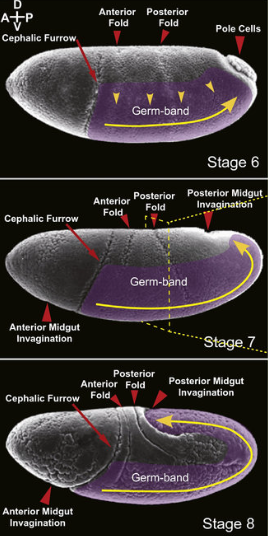
\includegraphics[width=\textwidth]{chapters/Results/figures/compareGB.png}
    \caption{A diagram of the germ-band and its motion (Source: \citeAY{kong2017forces}). The purple shaded area is the region of interest. }
    \end{subfigure}
     % \hfill
    \begin{subfigure}[b]{0.61\textwidth}
    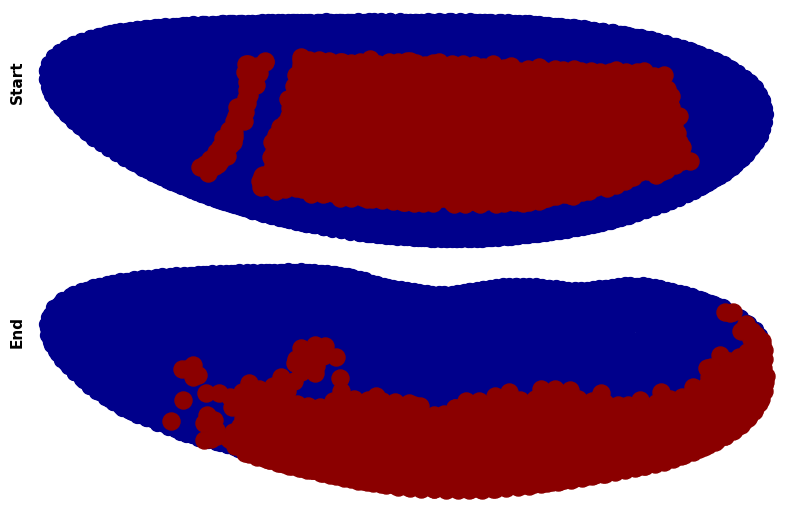
\includegraphics[width=\textwidth]{chapters/Results/figures/gb_firstframe_lastframe.png}
    \caption{Simulation with colored in germ-band at \\ $t = 0 \text{ min}$ and $t \approx 15 \text{ min}$\\Note: The blue line separating the germ-band in the initial frame is a quirk of the gene-expression-cutoff as described in Section \ref{App:morphogens}.}
    \end{subfigure}
    \caption{A visual comparison between a diagram of the germ-band cells and the cells as defined in our simulation\\}
    \label{fig:germbandCompare}
\end{figure}



To [reiterate], the motion of the germ-band is as follows:\\Firstly, the tissue moves downward towards the invaginating ventral furrow (\vf{A1}), then extends horizontally, and ultimately curve upwards as it encounters the back (posterior) tip of the embryo.\\

In general, we see great agreement between simulation and data in the final shape and placement of the germ-band, hinting that the movement towards the belly, back, and top side. This says nothing about the timing and [cooperation] of these [activities]. To get a better understanding of the agreement, we will need to look at the dynamics during this germ-band extension:\\

Later we will have quantitative measures, but for now, we can focus on a neat observation: The cells in the germ-band that start further towards the back will migrate much further horizontally than the cells closer to the head, with cells next to the \cephalic{cephalic furrow} only moving downwards (dorsally). \todo{Rephrase + make figure?} This is a result of the extension being the sum of many small contributions adding to the global motion. 

For a representation of the motion of individual cells in the germ-band, a random selection can be seen in Figure \ref{fig:GBMovements} below:
\begin{figure}[H]
    \centering
    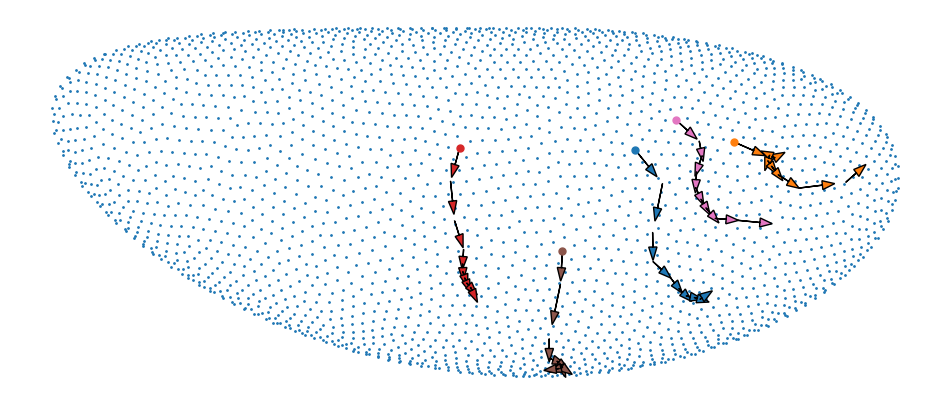
\includegraphics[width=1\linewidth]{chapters/Results/figures/movements.png}
    \caption{\todo{Remove some of the cells -- it's cluttered. Change color over time?}}
    \label{fig:GBMovements}
\end{figure}

It can be seen that we have captured the [unequal] cell migration, where cells that starts further along the horizontal axis along also moves more horizontally. 

For completeness sake, we have also made a stream-plot where, the flow field which is a way to visualize the individual motion of all cells at once. This can be seen in Figure \ref{fig:streamplot}:


\begin{figure}[H]
    \centering
    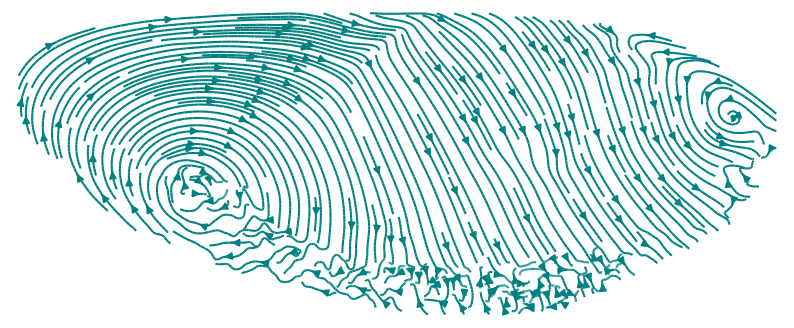
\includegraphics[width=1\linewidth]{chapters/Results/figures/streamplot2.png}
    \caption{\todo{make good?}}
    \label{fig:streamplot}
\end{figure}

Without any basis of comparison YYY.  but it looks cool.
Looking at the sum of these single-cell movements and behaviors can anyway give us a deeper insights into the global dynamics of the tissue.\todo{finish}\\

To summarize: We have a great visual agreement in the change of tissue-scale morphology of the germ band. The migration downwards towards the belly (ventral side) due to the furrow formation, the germ-band actuating horizontal motion, and finally the 'rise' at the back (posterior tip) due to the boundary condition, all seems to have been captured by the model. Through single-cell analysis we see a general correspondence between simulation and reality, [preliminarily] supporting that the tissue behaves as expected.\\  


An examination of the dynamical timeline will have to wait till later sections, but in general, we find that the morphological changes of the second main event, the germ-band extension (\gb{A2}), with reasonable hesitancy has been recapitulated.


\subsection{The Posterior Midgut Invagination (\pmg{A3})}
Now, this final point of focus is harder to visualize neatly. Looking at electron microscopy as below in Figure \ref{fig:PMG-IRL}, we can get a rough idea of the motion:
The back tip moves slightly upwards. Once it reaches a certain point, the tip folds in on itself as the ventral furrow reaches it, connecting the tube with the invaginating cavity. \textit{The Embryonic Development of Drosophila Melanogaster}

\begin{figure}[H]
    \centering
    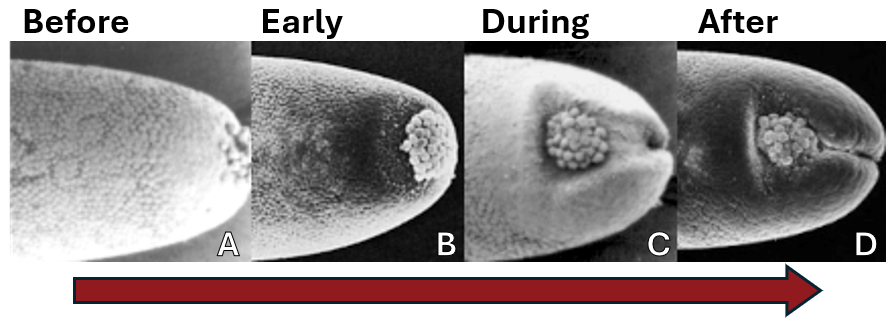
\includegraphics[width=1.\linewidth]{chapters/Results/figures/4stepPMG_annotated.png}
    \caption{An overview of the \textit{posterior midgut invagination} (\pmg{A3}) as viewed from the top (dorsal) side. \\The pole cells -- which are clearly visible at the posterior tip (\textbf{A})-- are moved to the top and towards the front of the embryo (\textbf{B}). As the tissue beneth them apically cinstrict, the newly formed indent merge with the \vf{ventral furrow} as this reaches the posterior tip (\textbf{C}). Finally the pole cells are internalized as the furrow closes off (\textbf{D}).The time points are not linearly [distributed].}
    \label{fig:PMG-IRL}
\end{figure}
Zooming in on the very back of our simulated embryo, we can see much of the same dynamics represented:
\begin{figure}[H]
    \centering
    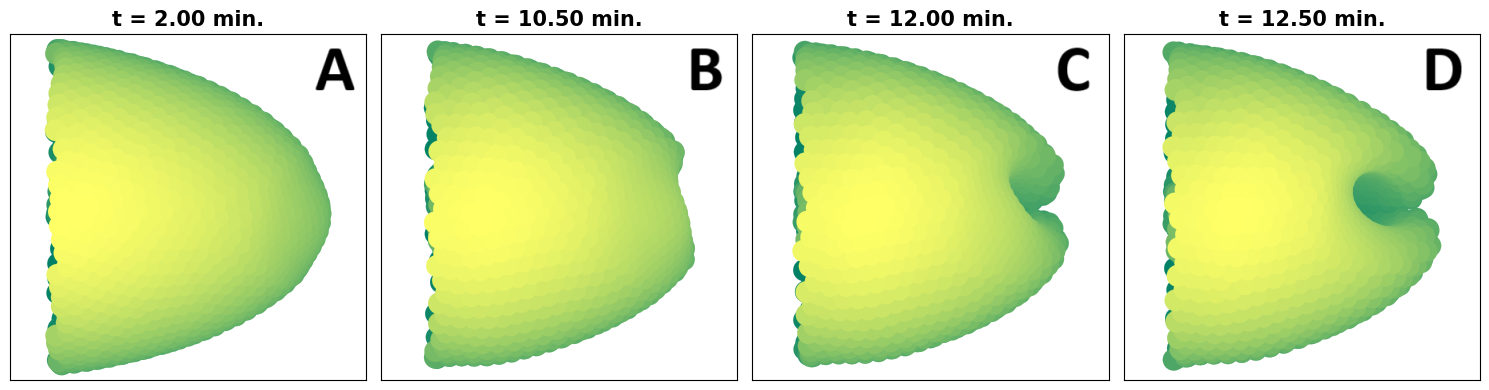
\includegraphics[width=1.\linewidth]{chapters/Results/figures/VisualPMG.png}
    \caption{A zoom-in on the the top side of the posterior tip of the embryo. To to be compared with Figure \ref{fig:PMG-IRL}. \\The PMG-event (\pmg{A3}) goes as follows: The cells in the tip starts tightening (\textbf{A}), the tip then is pushed upwards (\textbf{B}) and invaginates as the ventral furrow comes from below (\textbf{C}) before being moved further up (\textbf{D}) }
    \label{fig:visual-pmg-external}
\end{figure}

The formation of the \pmg{posterior midgut} is an intensely studied phenomenon in Drosophila gastrulation, but has, to the best of our knowledge, not previously been simulated. \todo{One more sentence}.

It can be hard to see what happens in vivo, as there is a distinct lack of good imaging of this phenomenon. This is likely caused by the [action] happening very quickly (the fold buckles as a release of pressure) and that much of the interesting cellular dynamics happens inside the embryo.\reph This point will return shortly, but visually we seem to be agreeing with the imaging for the most part. In general we capture the motion upwards followed by both a folding and a fusion. Unfortunately, in our simualtion the upwards momentum is slowed to a halt -- in vivo, the posterior is moved much further after invagination. Once again, the lack of pressure coming from the belly-region of the embryo seems to be to blame. \todo{mention dorsal folds?}\\

Our frustration with a lack of good reference images comes down to the fact that once invaginated, cells are impossible capture by ordinary microscopy and hard to focus \todo{finish sentence}. This is except for a single visualization of a meticulously \textit{hand-tracked} vertical band around the posterior tip. The approximate extend of this band can be seen here:\todo{explain slightly more}

\begin{figure}[H]
    \centering
    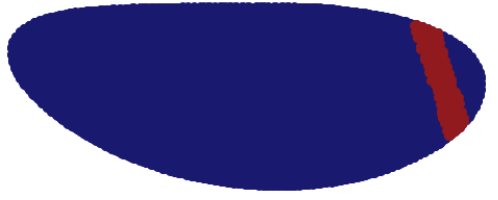
\includegraphics[width=0.5\linewidth]{chapters//Results//figures/daniel_band_pos.png}
\end{figure}

As looking 'inside' our virtual embryo is trivial compared to real life, we have extracted the band of cells, trying to recreating the framing of the data. In Figure \ref{fig:daniel-cells} the collected data can be seen and in Figure \ref{fig:comparetodaniel} an [imitation(?)] of the same cells can be seen in simulation. 
\newpage
\begin{figure}[H]
    \centering
    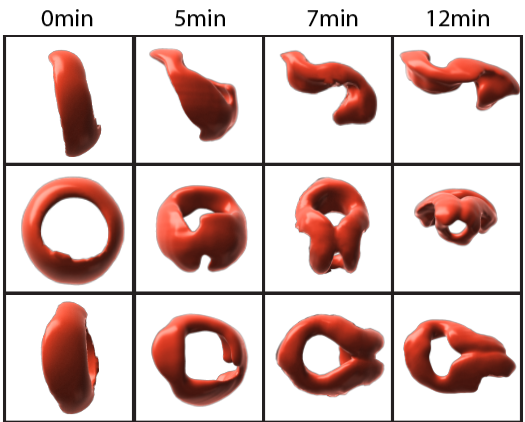
\includegraphics[width=0.7 \linewidth]{chapters/Results/figures/DanielCut.png}
    \caption{A 3d mesh of hand tracked cells from in vivo imaging. Each row is from a constant angle. (Source: Daniel Alber. Not yet published. Reproduced with permission)}
    \label{fig:daniel-cells}
\end{figure}
\begin{figure}[H]
    \centering
    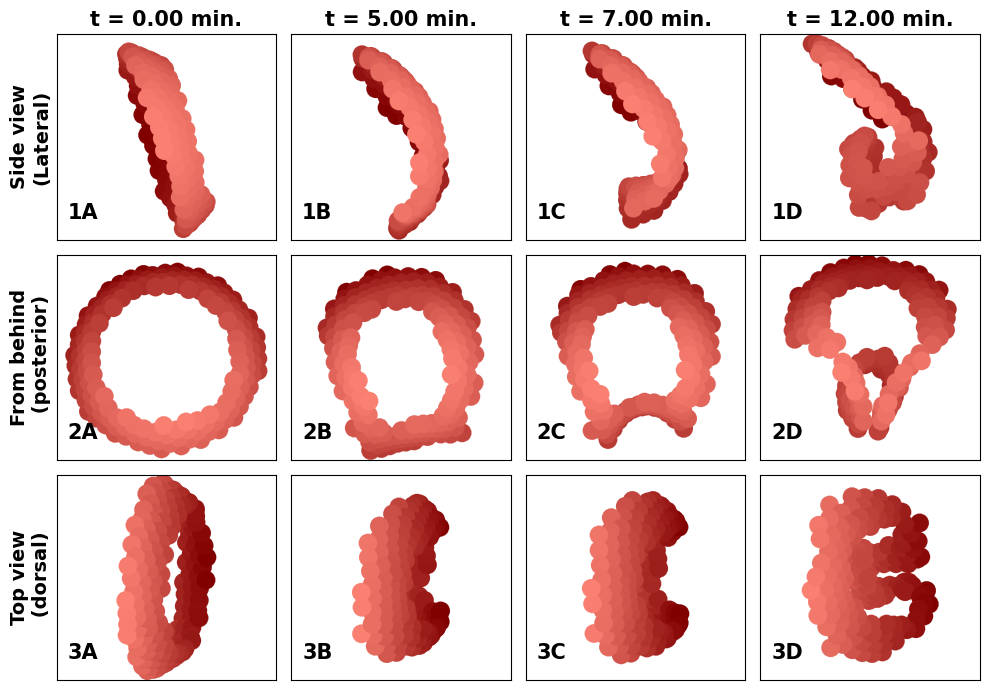
\includegraphics[width=0.8\linewidth]{chapters/Results/figures/CompareToDaniel.png}
    \caption{\todo{make cool 3D cells so it looks more like Figure \ref{fig:daniel-cells}?}}
    \label{fig:comparetodaniel}
\end{figure}

The combined invagination of the PMG and the ventral furrow (\pmg{A3}), is easily visible in \textbf{2C-}\textbf{2D}. For the first 5-6 minutes of the timeline, simulation and reality are relatively well aligned. We see a push from the extending germ-band moving the cells towards the posterior tip. The trouble begins in \textbf{1C} and \textbf{1D} where the orientation of the cell-band should be almost horizontal. As Figure \ref{fig:comparetodaniel} shows, our model has not moved the cells far enough towards the top. In spite of this, as the posterior closes off, a YY right morphology emerge. It should also be noted that the closing happens at a reasonably YYY timing. In general a we have a respectable qualitative agreement, albeit the trouble the lack of upwards (dorsal) motion is visually evident.\\



Our model clearly has some fundamental flaw or inconsistency, but barring the lack of movement towards the back, we got quite close in both timing and shape. With a few exceptions, our model provides a phenomenologically faithful recreation of this vital morphogenetic event. As the posterior invagination (\pmg{A3}) requires both successful modeling of (\vf{A1}) and (\gb{A2}), we are, to the best of our knowledge, the first group to attempt an in silico [experiment]. So while our simulation is not perfect, the fact that this is a world-first attempt at something this well-studied is a  noteworthy [achievement(?)].\\

\todo{reread these last two paragraphs. I feel like I am rambling}
 

\subsection{General morphology}
In the literature, a common way of visualizing changes in both local and global structure, consist of virtually drawing straight lines on an embryo at the onset of gastrulation. How these lines translate and skew over time is very descriptive for how the form changes. An example in both data and simulation can be seen in Figure \ref{fig:band-movements-stas}.

\begin{figure}[H]
    \centering
    \makebox[\textwidth][c]{\hspace*{-1cm}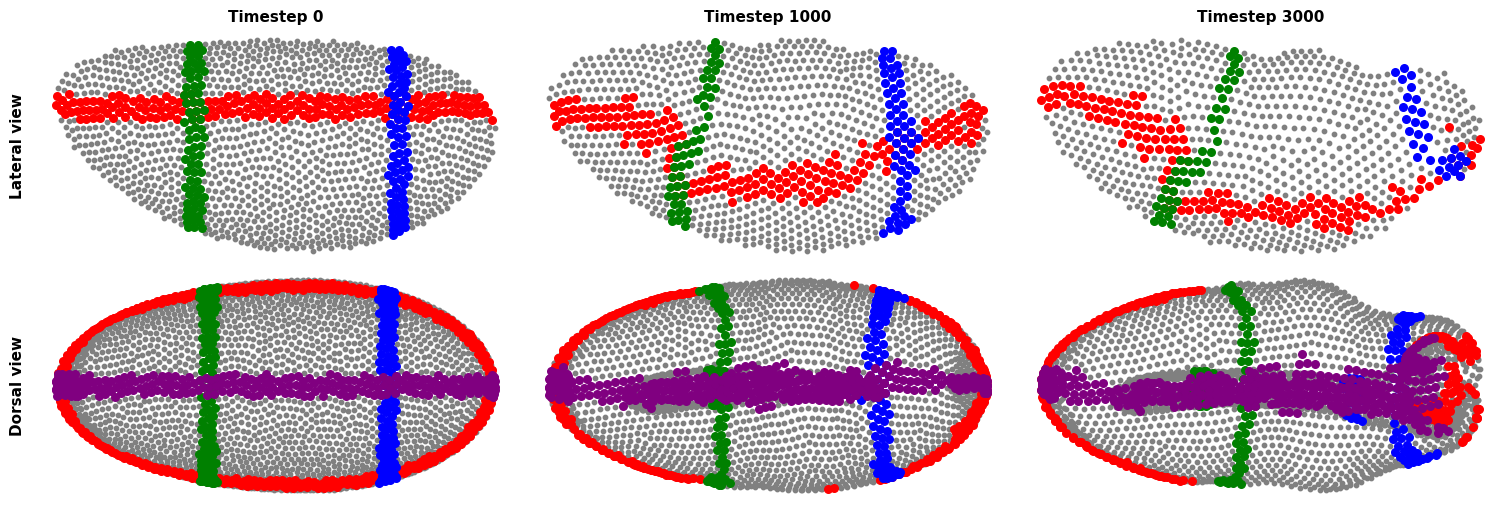
\includegraphics[width=1.\linewidth]{chapters/Results/figures/band_movements.png}}
    % \caption{My simulation. Compare to figure \ref{fig:band-movements-stas}}
    % \label{fig:band-movements}
\end{figure}
\begin{figure}[H]
    \centering
    \makebox[\textwidth][c]{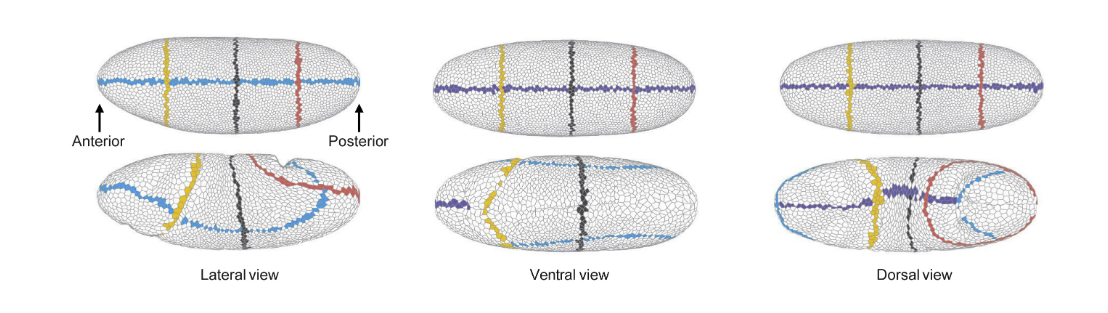
\includegraphics[width=1.\linewidth]{chapters/Results/figures/compareStasGBShape.png}}
    \caption{Positions of specific bands over time. \\ \textbf{Top row:} Simulation. Three time steps from two different angles.\\ \textbf{Bottom row:}  Segmented images (Source: \citeAY{stern2022deconstructing}). \\\todo{write more!}}
    \label{fig:band-movements-stas}
\end{figure}

This juxtaposition allows for some interesting observations:\\
As is evident, there is a general agreement between both local and large-scale changes in embryonic form. \\

Going through the lines, color by color we might be able to surmise [smth] about the differences in dynamics between our model and [in vivo]:\todo{finish}

\begin{description}
   \item[\lightblue{Blue}] The biggest problem is also very evident plaguing our simulation is evident. The pressure from the bottom (ventral) side of the model cannot YY. The blue line acts as a stand-in for the germ-band. Much of the analysis from its section applies with two exceptions:
   \begin{itemize}
       \item In simulation, close to the (deliberate) lack cephalic furrow (the \lightyellow{yellow} line), the blue line breaks up. \todo{write something about lack of pressure relief}   
       \item The second image is later than what we previously compard the germ-band to. Here the lack of upwards motion is (much like all the woke left) pronounced.\todo{make professional}
   \end{itemize}
   \item[\lightred{Red}] The same effect can also be seen in the red line, where it almost, but not [totally] reach the rightmost (posterior) tip. It can also be seen, that after invagination and the lines close to the end (red and blue) becomes muddled.
   \item[\lightyellow{Yellow}] A helpful line for understanding the motion around the area of the cephalic furrow. The top part moves towards the bacj and the bottom towards the front. Not too much bending. We have great agreement! 
   \item[\lightpurple{Purple}] The mid-line seems as stable as in vivo. The "bunching up" of the \lightpurple{purple} in the posterior-end is most likely an artifact from the fact, that -- unlike in real life -- the cells are not being hidden below other tissue in the posterior invagination.
\end{description}


fault lines er godt ord

We will discuss this later, but a possible root of the problem is also a lack of flexibility in the top (dorsal) tissue. This most likely stems from a lack of [Dorsal Transverse Folds]. \todo{finish though, mention pre-print?}

Other observations:
The point cloud of our 'cells' become spread out in a way that mirrors the individual cells quite radical surface area increase after room has been made by the various invaginated tissue. 


Quickly summarizing all the qualitative comparisons we have seen in this section: We have found some surprisingly great agreement! From the full embryo comparison in Figure \ref{fig:big-visual-comparison} and the individual events, the gastrulation seems to qualitatively have been recuperated well, both in timing, in the intermediate morphologies, and in the resulting structural shapes.


\todo{transition?}
% \subsection{Daniel}
% \todo{Make use of section or cut}
\section{Quantitative Agreement}

While visual inspection of our simulation is interesting -- and is a clear result in itself, given that morphology is the target -- we would like some quantification of the model performance. 

Having a numerical framework would allow for optimizing model parameters, performing parameter sensitivity analysis, and in other ways objectively defining the accuracy of our solution. It also allows for statistical checks on the consistency between simulation and experimental data, helping to quantify the degree of alignment between the two. Additionally, this framework would provide a foundation for testing various hypotheses regarding cellular behavior and tissue mechanics, ultimately leading to more robust YYY of models and insights maybe into the underlying biological processes.


To remind ourselves, we set out with a handful of core [inquiries]. First, we wanted to determine the minimal set of rules necessary for 'in vivo-like' gastrulation to [emerge]. Next, we aimed to explore whether the boundary and initial conditions alone are sufficient to drive these processes i.e. whether the interplay and timing that [stretch] multiple minutes were a results of [something else]. Finally, with a (hopefully somewhat validated) bottom-up\todo{explain}, full-scale model in hand, we sought to understand what insights could be drawn about the interaction between domains.


\\
We will now take a step back from the individual morphological events and focus on large scale analytics.

It was stated earlier that quantitative data is tough to come by. But very recent technical advancements in microscopy and cell-segmentation has given rise to the possibility of large-scale, automated analyses.\cite{stern2022deconstructing} We will take our onset in data collected in \citeAY{stern2022deconstructing}. The data-set consist of machine-tracked cell positions in 3d-space.

We will now go through \textit{quantitative} explorations of the agreement between our model and data collected in vivo. 


\subsection{Movements}

Even though the outcome of a successful morphogenesis of course is a three-dimensional shape, it is the dynamics of the system we are interested in recreating. As there is no canonical way of labeling the cells, we have no way of doing any one-to-one cell comparisons. Therefore the following measure was devised: 

Take each simulated cell and find the average displacement vector of the 10 spatially closest cells in data:

\begin{equation}
    \boldsymbol{\mu}_i(t=\tau) = \frac{1}{N} \sum_{n=1}^{N}\boldsymbol{v}_n(t=\tau)= \frac{1}{N}\sum_{n=1}^{N}\left(\boldsymbol{p}_n(t=\tau) - \boldsymbol{p}_n(t=\tau-1) \right)
\end{equation}
Where the sum over $n$ is for the N nearest in-data neighbors of the simulated particle $i$ at time step $\tau$.

Now also calculate the displacement of the particle $i$$\boldsymbol{v}_i$ since last time-step. This way we can find the angle between the cells motion and the "average motion vector" of a in-vivo cell at this position:
\begin{equation}
    \alpha_i(t=\tau) = \arccos\left(\boldsymbol{v}_i(t=\tau)\cdot\boldsymbol{\mu}_i(t=\tau)\right)
\end{equation}

The resulting (acute) angle difference is between 0 and $\pi$. 

Below (in Figure  \ref{fig:motionAgreementExample}), the resulting analysis can be seen, were each motion vector is colored according to their agreement with the data.

\begin{figure}[H]
    \centering
    \makebox[\textwidth][c]{
    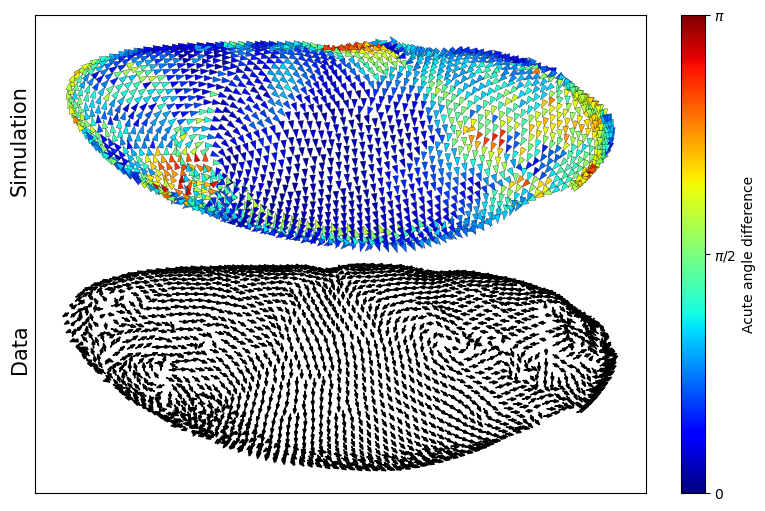
\includegraphics[width=0.9\linewidth]{chapters/Results/figures/movement_vectors_example.png}
    }
    \caption{Snapshot of motion vectors for each cell in simulation and average motion at each cells position. \todo{larger label to colorbar, write time point somewhere}}
    \label{fig:motionAgreementExample}
\end{figure}


It can be seen that at this specific time point, the agreement ranges from surprisingly good to predictably bad. 

We Convergent extension is by its very nature based on the global motion being being different from the motion of the individual (see Figure \ref{fig:ConvergentExtensionDiagram}). Having a per-cell agreement is almost contradictory to this type of cell motility. 





Finally, for ease of parsing, we scale this number to be between 1 and 0, allowing us to score the particles motion at this point in time:

\begin{equation}
    \xi_i(t=\tau) = 1-\alpha_i(t=\tau)/\pi
\end{equation}

This should hopefully give us an estimate of the agreement to the general kinematics for the different cells.


Averaging this score over the whole embryo for every time point we get the following relation:

\begin{equation}
     \Lambda(t=\tau) = \frac{1}{N_{cells}} \sum_{i=1}^{N_{cells}}\xi_i(t=\tau)
\end{equation}
In Figure \ref{fig:motionAgreement}, the $ \Lambda$-measure can be seen for different points of time in the simulation:

\begin{figure}[H]
    \centering
    \makebox[\textwidth][c]{
    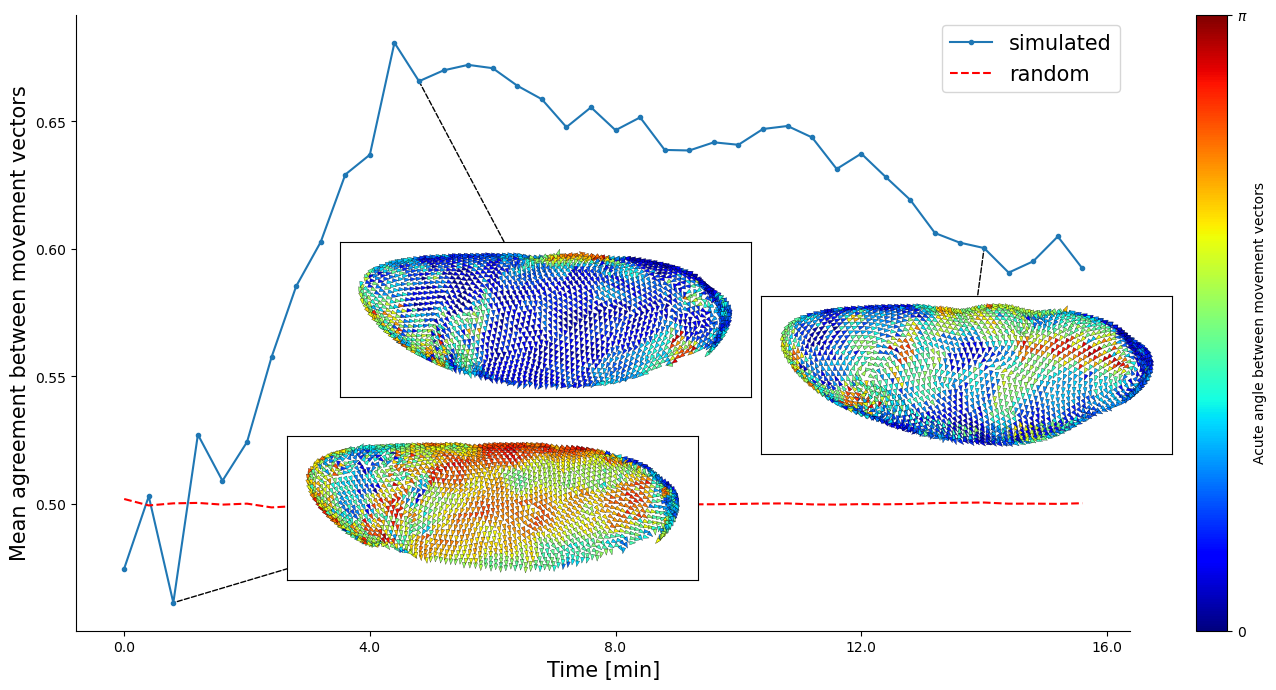
\includegraphics[width=1.3\linewidth]{chapters/Results/figures/movement_vectors_normal.png}
    }
    \caption{The average motion-vector agreement across the full embryo as a function of time\\
    The red \textit{random}-line is a simulated embryo where every direction of motion is uniformly randomly chosen. \todo{explain x-axis}}
    \label{fig:motionAgreement}
\end{figure}

\todo{describe \textit{random}}

In general, we see a consistent, well-above random overlap between data and simulation. 

From the previous sections, we had some intuition that our simulation visually followed the general flow of the morphogenesis. Figure \ref{fig:motionAgreement} gives us some quantitative confidence that the motion of the individual cells also align with the data. However, subtle differences in mechanical properties between the simulated and actual cells must be accounted for to fully capture the dynamics of this process. Specifically, biological cells exhibit a degree of elasticity and plasticity that is not fully represented in our model.

It is very clear that in the first couple of minutes our simulation and reality does not completely agree. This will be a recurring theme. We believe this is cause by the fact that in nature, the cells are more elastic in real life than in simulation. When the \vf{ventral furrow} invaginates, the pulling for needs some time to stretch the tissue. In our model, the sides moves down immediately and uniformly. Adding explicit cell shape changes might allow for more gradual stretching allowing the cells to adjust to tensile forces. We hope, that a more realistic tissue flexibility could help address these early differences between the simulation and what has been observed in vivo.


We will now be looking at the integrated error over the full run.

\begin{equation}
     \Lambda_i = \sum_{\tau = 1}^{N_t}\xi_i(t=\tau)
\end{equation}

Mapping the resulting "average lifetime error" back onto the initial positions we can see how the error is spatially distributed:
\begin{figure}[H]
    \centering
    \makebox[\textwidth][c]{
    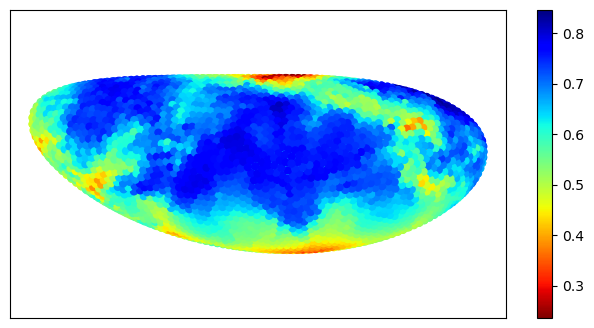
\includegraphics[width=0.8\linewidth]{chapters/Results/figures/movement_mapped_normal.png}}
    \caption{The motion-vector agreement across the full run mapped back onto their original positions \todo{colorbar label}}
    \label{fig:}
\end{figure}

The in silico motion of the germ-band seem in great agreement with data, especially given how far the individual cell travels. This alignment reinforces the validity of our model for large-scale cellular movements, particularly for cells located on or around the \gb{germ-band}. The match in overall trajectory and displacement at least highlights the model's ability to capture the large-scale observations.\\
Because of the way the imaging was done, all invaginations (the ventral furrow for example) will automatically have low agreement. The original data only supported motion-tracking on the exterior surface of the embryo.  This limitation naturally reduces the precision of our comparisons in regions where inward movements are critical, like the ventral furrow. This can also be seen on the top (the dorsal side), where the sheet buckles and folds in nature. This was not part of our simulation and it can also be seen that our measure of agreement are penalized.\\
Also, the anterior (head) part of the embryo was pretty early deemed outside of scope of the current project and any agreement there stems purely from our generic(?) model.\\

This all gives us the idea of looking at the agreement for specific parts of the egg.



\begin{figure}[H]
    \centering
    \makebox[\textwidth][c]{
    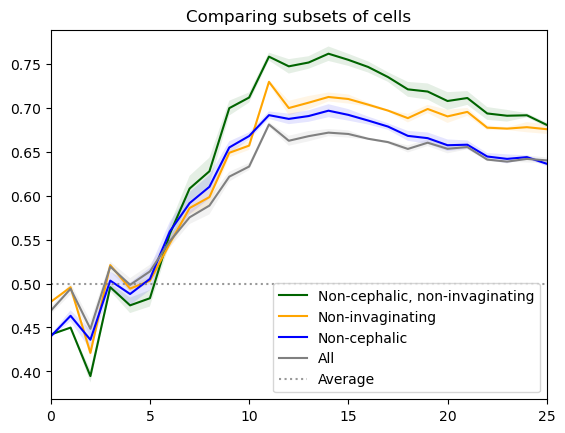
\includegraphics[width=1\linewidth]{chapters/Results/figures/movement_vectors_normal_subsets.png}}
    \caption{The motion-vector agreement across the full embryo as a function of time. For confidence is the stability of the current solution, all lines and shaded areas are averages and and standard deviations of three runs using identical parameters but different seeds.}
    \label{fig:vector-subsets}
\end{figure}

In Figure \ref{fig:vector-subsets}, we tried limiting the agreement analysis to only look at subsets of the embryo:

Once anything in the head area was discard from the average (Non-cephalic), we see a noticeable bump in quality. This is true for the most of the duration, but the effect is actually reversed in the far ends of the simulation. We believe this occurs because of the relatively well-behaved cephalic region --  excluding it helps boost the overall average when other regions perform well. However, when the rest of the simulation decline, removing the head slightly heightens the average quality. 

Removing cells in the Ventral and Posterior areas that were apically constricting (Non-invaginating) we see an even more pronounced increase. This time, the increase is, predictably, more stable, as these areas are responsible for consistently worse performance. Without the complicating influence of these invaginating cells, the remaining regions track more closely with the motion data, leading to a better  agreement

Combining both masks (removing both the head-regian and the  invaginating parts) gives an exponentially better [something averages]


Focusing on the parts of the embryo with a good possibility of overlap with data, we have a much higher average cell-motility agreement (almost 0.8), especially during the most dynamic phases of the simulation. The improvements are substantial and we feel it helps portray how our model can excel.



\todo{Just realized I did not remove the invaginating pmg int the "Non-invaginating" part. I am dumb as a doorknob}


\subsection{Timing}
One of the key question we propose is whether precise timing mechanisms are necessary to drive the complex morphogenetic processes we see, or if they can emerge purely from initial conditions and cell interactions.\\
Cells have been shown to have remarkably precise internal clocks\footnote{cool footnote with a remarkable number\cite{cellinternal}} and chemical gradients in the embryo changing across timescales from seconds to hours\cite{shvartsman2008dynamics}. There is also the "biological clock"\cite{johanolsen2} that proteins themselves have dynamic structure that can change over time.\cite{johanolsen1}. But there is no evidence for any specific timing in stages 5-7 [citation needed]. We would like to stress the importance of the result that we seem to have recapitulated some of the long-term dynamics completely without any explicit time-dependent parameters. \textit{The fact  that the processes can exhibit accurate emergent behavior through local rules, rather than requiring external temporal control. }This could be seen to corroborate our thesis that initial conditions and an inter-cellular rule set is sufficient for some of natures more complex morpologies to arise. 

\subsection{Strain}
As the tissue warps and skews, the cells are both subject to- and drivers of- stress and strain on the cell walls. This is one of the most widely studied parts of structural changes in morphogenesis.

While our simulation neither includes cell walls nor explicit strain calculations, a method has been developed that only requires positions of cell-centers -- and that we have! The Green-Lagrangre algorithm (implemented as described in \citeAY{butler2009cell}), can be applied to find local deformations in tissue. In Figure \ref{fig:strain} the results of an implementation can be seen and compared to a graph on data.

\begin{figure}[H]
    \centering
    \begin{subfigure}{0.45\linewidth}
        \centering
        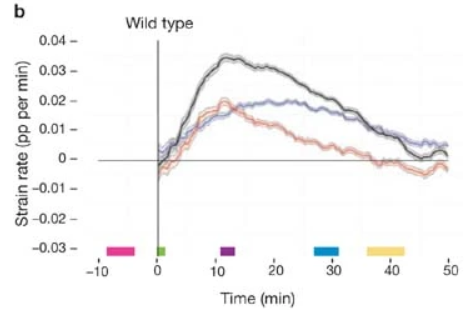
\includegraphics[width = \linewidth]{chapters/Results/figures/strain_rate_extrinsic.png}
    \end{subfigure}
        \begin{subfigure}{0.45\linewidth}
        \centering
        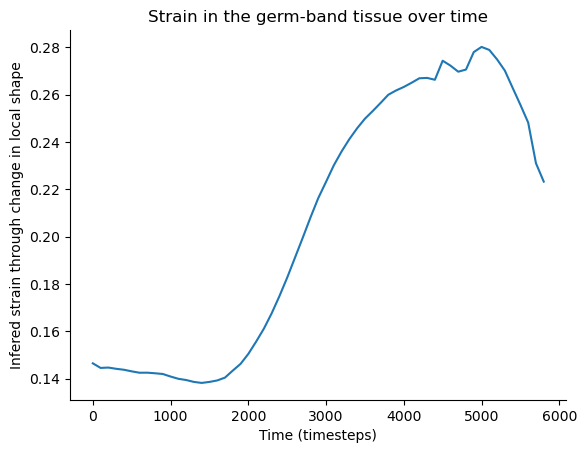
\includegraphics[width = \linewidth]{chapters/Results/figures/strain_smoothedpng.png}
    \end{subfigure}
    \caption{(Source: \citeAY{butler2009cell}) (\textbf{left}) and the inferred strain in our simulation (\textbf{right}).\\
    We both see a quick rise followed by a fall-off at time of invagination of the posterior\\\todo{Explain the leftmost plot or find another that shows the same with only one line}}
    \label{fig:strain}
\end{figure}

In the first 12-15-minutes we see a rising strain, ending at the point of internalization of the germ cells ($\approx12$minutes). In our simulation, the strain has a delayed onset, once again showing how the first 2 minutes have a central difference from ground truth. To remind, we previously postulated this was due to overly rigid tissue in simulation, which would also explain the failing strain calculation. \\

This section was kept in for comparison purposes, as it highlights a fundamental discrepancy in tissue mechanics between our model and actual biological behavior.  

We see, despite the overall success of the simulation, this divergence in strain accumulation further suggests that the mechanical/viscoelastic properties of the tissue are not fully captured and might require further refinement. 


\subsection{Ventral Furrow}
I would love to quantify the accuracy of our simulated ventral furrow.\\
I am guessing we can do a cell-center fit of Figure \ref{fig:VFComparison}.\\
Is this out of scope? Yes. Would it be cool? Also yes.

\subsection{Cell surface area}
I am sure I could get the data and would love to quantify the agreement.
I am guessing we can do a neighbor-distance measure.\\
Is this out of scope? Yes. Would it be cool? Also yes.
\newpage
\section{In Silico Mutants}
\todo{Give me all the questions again}
Having a complete simulated pipeline from (simplified) morphogen to (approximate) morphogenesis, opens the door for some intriguing explorations into our model and its relation to nature. \\

A large branch of developmental biology consists of discovering or creating mutated genotypes and cataloging the resulting organisms. 
Our model also allows for the creation of genetically-variant embryos by changing the response to one or more of the simulated morphogens. In theory, we can make \textit{predictions} by analyzing how variations in morphogen distribution or cell interactions affect morphogenesis in our simulation. We might be able to gain insights that could inform or direct experimental studies.\\

To introduce this section we will need to shortly explain the most interesting "mutants" that incidentally hinder \vf{A1}, \gb{A2} and \pmg{A3} respectively. The mechanics, morphologies, and implications for our model will be explored. 

\subsection{The mutants}


\subsubsection{No Ventral Furrow (\vf{A1})}
When knocking out the \textit{Twist} and \textit{Snail} genes, which are primary organizers of apical constriction,he ventral furrow fails to form (stage \vf{A1} on Figure \ref{fig:big-timeline}).\cite{leptin1991twist} t

The resulting embryo does not move the germ-band downwards, making the pressure exerted by this unable to move the posterior "upwards". This can be  seen in Figure \ref{fig:VFmutant}.\\

\todo{Make figure}

The resulting embryo does not move the germ-band downwards initially, which delays the pressure exerted by this movement. In real life, after a delay, the system is overdetermined and other actions overtakes to eventually shift the posterior upwards, allowing the process to proceed. Interestingly, even with this altered timing and mechanical dynamics, the posterior region still manages to achieve its upward shift, and the embryo often remains viable.\cite{conte2012biomechanical} This suggests that while the normal motion provides an optimal pathway for development, the system has enough flexibility to accommodate deviations and still reach a functional outcome.

\todo{cite \citeAY{lye2024polarised}}

% \url{https://genesdev.cshlp.org/content/5/9/1568.full.pdf}
% We are seeing the right thing
% Comparing We are seeing the right thing.



% \subsection{Auxiliary(cephalic furrows}

% In the absence of controlled folding of the dorsal tissue, the pressure from the extending Germ Band, can lead to other folds(?) \url{https://brunovellutini.com/posts/cephalic-furrow-thread/}

% This is key to both understanding why the invaginated posterior end does not travel further anteriorly.

% Also the large scale morphology change some runs had.

\subsubsection{No active intercolation / germ-band (\gb{A2})}
\label{sec:mutantNoGB}

When removing the patterning that is believed to be responsible for convergent extension in the germ-band, something surprising happens. It has been show that drosophila morphogenesis is driven by more than convergent extension, and \gb{germ-band}-mutants are still viable. In \citeAY{butler2009cell} they show that active cell elongation overtakes the resopinsiblity for moving the tissue.

In our simulation, we have no cell shape change to help alleviate the lack of motion, but as the ventral furrow still invaginates and expands we still see some movement as the invaginations pull on the sorrounding tissue. (Figure \ref{fig:germ-band-mutant})

\todo{Make figure}

\todo{conclude?}

\subsubsection{No Posterior Midgut (PMG) \pmg{A3}}
The PMG is the name for the invagination that happens at the posterior to internalize the pole cells (\pmg{A3} on Figure \ref{fig:big-timeline}).

In [cite Stas], they show that the chemical signals produced by the protein \textit{Hkb} initiates apical constriction around the posterior tip. In \textit{Hkb}-deficient mutants the lack of posterior invagination has a clear effect: The built up pressure from the extending germ-band causes the whole epethilium to twist. This has given the \textit{Hkb}-mutant the nickname "Corkscrew".\\

In Figure \ref{fig:corkscrew-comparison}, a video of the corkscrew mutant can be compared to our simulation after removing the cells ability to react to \textit{Hkb}.

 
\begin{figure}[H]
    \centering
    \makebox[\textwidth][c]{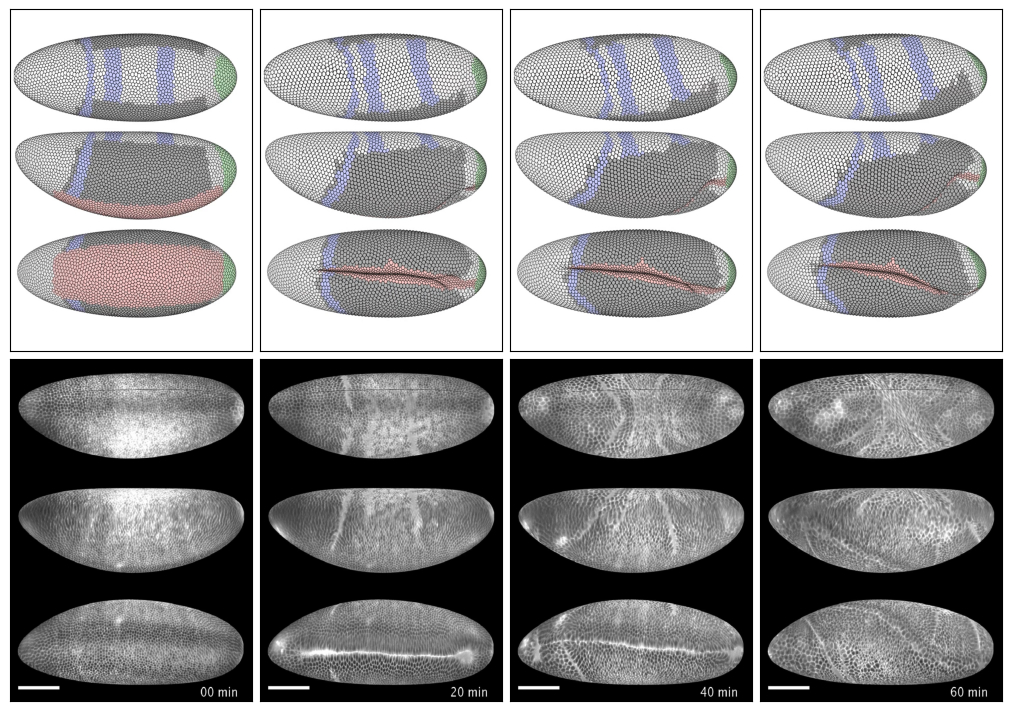
\includegraphics[width=1.2\linewidth]{chapters/Results/figures/corkscrew_comparison.png}}
    \caption{A purely visual comparison between our simulation \\
    \textbf{Top:}) and the \textit{Corkscrew} phenotype \\
    \textbf{Bottom:} \todo{describe}  (Source:\citeAY{smits2023maintaining}).\\ In both cases we see a "twisting" motion.}
    \label{fig:corkscrew-comparison}
\end{figure}
% Twist and shout

Comparing the lines formed by the ventral furrow on the belly of the embryo, we can see twisting phenomenon closely agree between the in vivo and in silico models, suggesting that the general tissue deformation dynamics are well captured by the simulation. The in vivo and in silico mutant visually agree on the motion, albeit on different time scales. Despite these timing differences, the key morphological features—such the furrow formation also remai consistent, hinting to robust underlying mechanisms shared between the systems.


Comparing the reaction of these in silico mutants to real life phenotypes gives us a hint that our model is capturing something fundamentally correct about the principles governing the cellular behavior. 

% This suggests that the broader processes driving morphogenesis may rely more on spatial and interaction rules than on precise timing."

% We know that \textit{Runt} and \textit{Even skipped} are upstream . The litterature is conflicted, but the general theory is, that the patterning allows for a coherent orientation of the planar cell polarity. 

% PCP-orientation was set at the intial step of the simulation as pointing in the distinct direction defined by the interspersed \textit{Runt} and \textit{Even skipped} patterning.
% The results are interesting, albeit very uneventful, as
% In the litterature  \cite{butler2009cell} more the morphogenesis is driven by more than Convergent Extension, and unstriped mutants are still viable, unlike our case where nothing happens.

% Seems to be a clear indicator for active cell shape change being a vital part of... 

% TODO: Discuss level of abstraction in the model 

\subsection{Combining and comparing to each other}


Given that we have the world’s first [citation needed] full embryo model, we can conduct some interesting in-silico experiments. A particularly fascinating aspect of morphogenesis across all species is the interplay between the various spatially separated dynamic regions of the embryo. In this section, we will analyze how these regions interact and influence each other and the final outcome.

We will be doing this analysis in two ways: Firstly by comparing the different virtual 'phenotypes' to our baseline model. Secondly by comparing to the motion data as used in earlier sections. Finally we will be making an interaction-matrix, quantifying the resulting compromises and cooperation.  
\todo{Fuck, cut for time}
\subsubsection{Pole Cell Migration}
We will start out by introducing the metric \textit{Pole Cell Migration} as a virtual quantification for the success of the gastrulation. The Pole Cell Migration is defined as the angle change of the posterior tip in the lateral plane. That is, in degrees, how far around the embryo the posterior has moved.\todo{make figure?}\\



In Figure \ref{fig:PCM-mutants} a comparison of multiple runs of the known mutants described earlier can be seen and compared to the wild-type.

\begin{figure}[H]
    \centering
    \makebox[\linewidth]{
    \begin{subfigure}[t]{0.9\linewidth}
            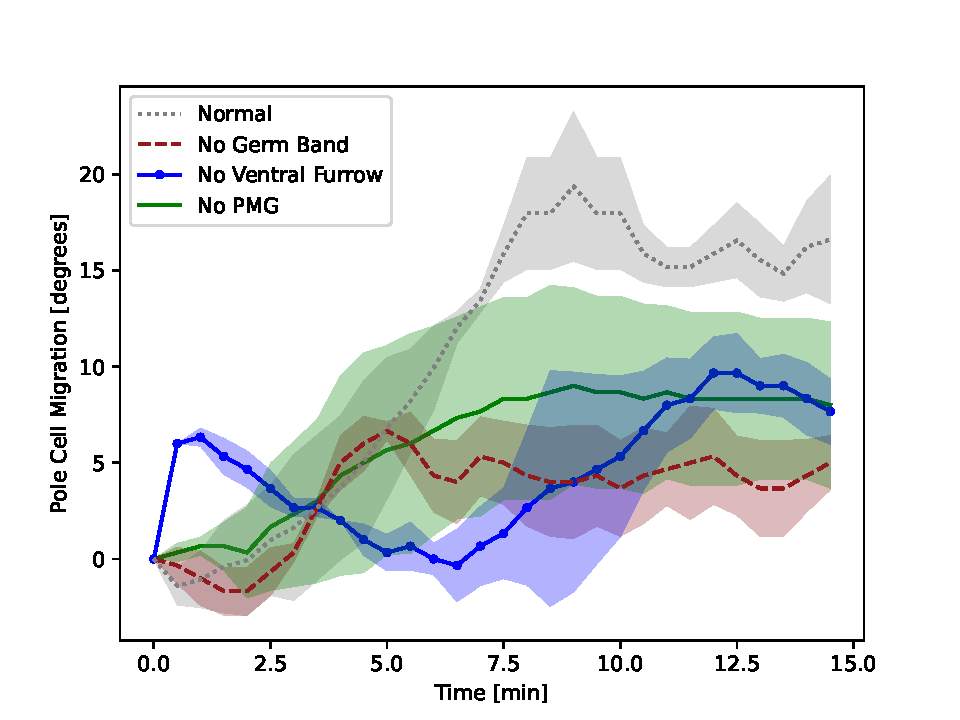
\includegraphics[width=1.\linewidth]{chapters/Results/figures/compare_PCM.pdf}
    \end{subfigure}
    \hspace{-1.2cm}
    \begin{subfigure}[t]{0.45\linewidth}
    
            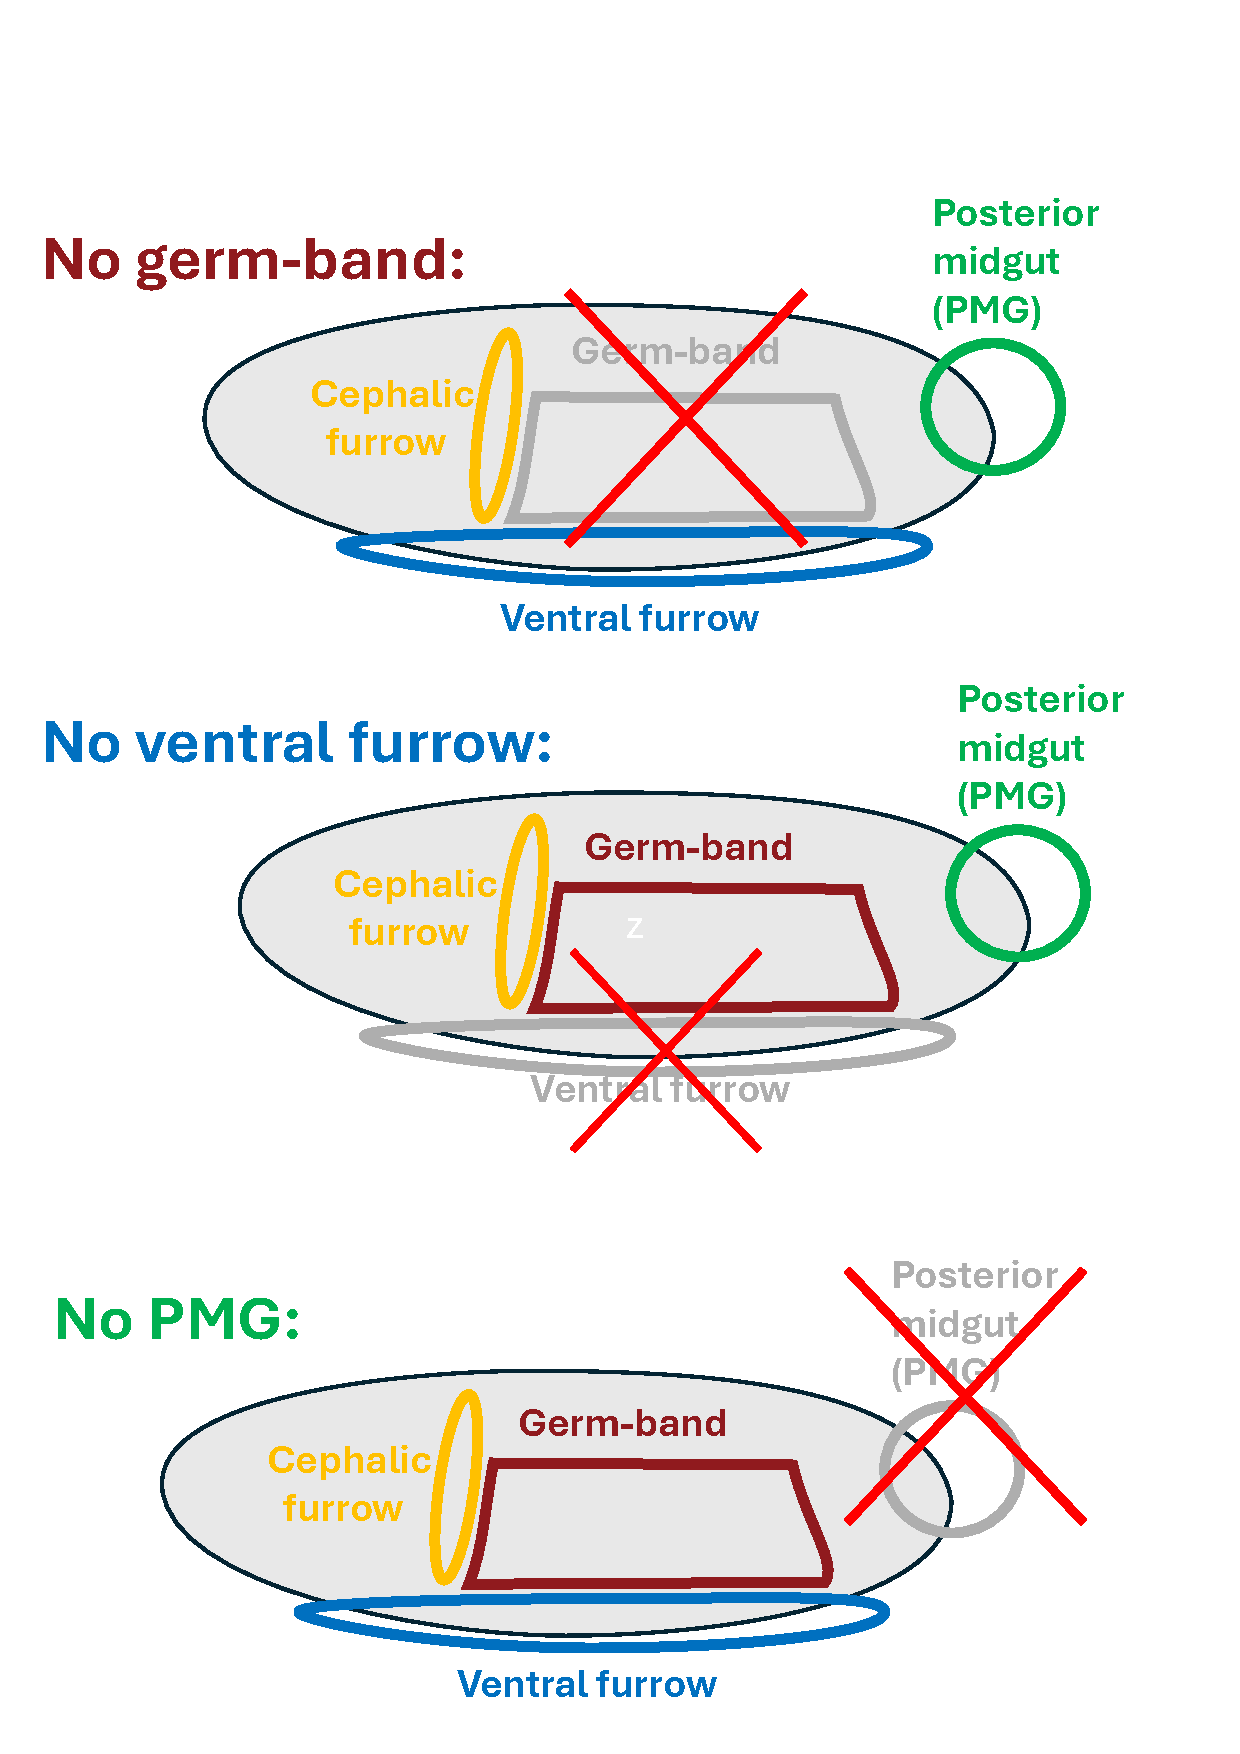
\includegraphics[width=1.\linewidth]{chapters/Results/figures/mutant_diagrams.pdf}
    \end{subfigure}
    }
    \caption{\todo{Explain,}}
    
    \label{fig:PCM-mutants}
\end{figure}


Videos of the individual runs can be found in Section \ref{App:videos} in the Appendix, but a lot of the dynamics of the system can be gathered from the motion of the posterior tip. We can see that:\\
\textbf{Normal (red):} This is the normal run. A ramping movement until reaching the point of posterior invagination at about just below 20 degrees. \\
\textbf{No Germ-band (green):} At first the tip moves towards the invaginating ventral furrow. As this expands slightly there is still a tendency to move the tip dorsally, but there is not enough force for the posterior tip to progress more than 5 degrees. \\
\textbf{No Ventral Furrow (blue):} Firstly, when no tissue is pulled into the ventral side, the germ-band pushes the posterior tip slightly upwards. This is negated as the pressure ultimately comes from the 'port' and 'starboard' sides, not translating the pole cells upwards.\\
% \begin{wrapfigure}{l}{0.\textwidth}
%     \centering
%     \hspace{-3cm}
%     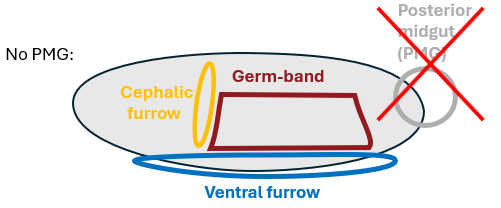
\includegraphics[width=0.5\linewidth]{chapters//Results/no_pmg_mutant_schematic.png}
% \end{wrapfigure}
\textbf{No PMG (yellow line):} Here we see a possible breakdown of this metric. None of the corkscrew-twisting is captured and the lowering of PCM does not capture just how unviable an embryo with this mutation is.  


\subsection{Combining and comparing to data}
While comparing internally is interesting and can say a lot about the dynamics, we wanted a short detour where we recreate Figure \ref{fig:motionAgreement}, seeing how each mutation changes the motion-vectors. The results can be seen in Figure \ref{fig:compare-motionAgreement} below:

\begin{figure}[H]
    \centering
    \makebox[\textwidth][c]{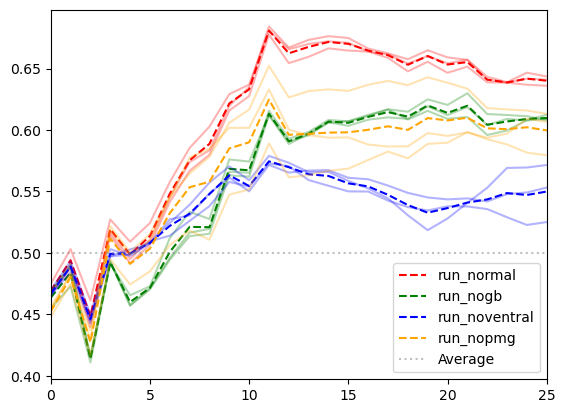
\includegraphics[width=1.3\linewidth]{chapters/Results/figures/PLACEHOLDER_compare_movement_vectors.png}}
    \caption{ Y-axis defined like Figure \ref{fig:motionAgreement}. \todo{This is an important plot. Remake in higher quality with  better legend and axis labels}}
    \label{fig:compare-motionAgreement}
\end{figure}
It is comforting to see that the motions are 
\todo{Find something interesting to discuss}

The "No Germband"-mutant is surprisingly good. We think this is due to the fact that only the angles between the motions matter: If the cell-sheet moves along the right direction, it does not matter whether they move far enough.   

But when are the different parts important? To figure this out we have the following figure:

\begin{figure}[H]
    \centering
    \makebox[\textwidth][c]{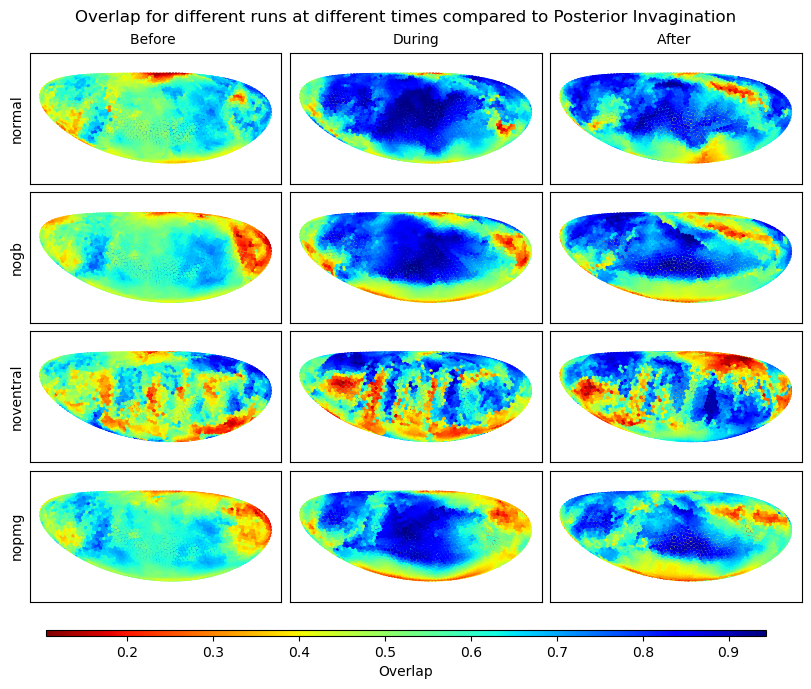
\includegraphics[width=1.3\linewidth]{chapters/Results/figures/Compare_all_movements.png}}
    % \caption{This is the main plot of the thesis. Y-axis is sum of y-axis of over all times in Figure \ref{fig:motionAgreement}}
    % \label{fig:compare-motionAgreement}
\end{figure}
\todo{I feel like there is a lot of meat on this figure. Discuss!}

\textbf{We are in a way the first who can simulate the posterior invagination (PMG) \pmg{A3} as this requires both successful modelling of \vf{A1} and \gb{A2}. Each of which has had multiple YYY before, but never in a way where combining them was possible}?
\section{Interaction Matrix}
For a more granular approach, we boil the PCM down to a single number quantifying the total dorsal motion. In the matrix in Figure \ref{fig:PCM-matrix} the combined effects of missing any two can be seen (once i make it) together with the data-quantified overlaps:
% \footnote{emitting about 7kg of CO2 \url{https://mlco2.github.io/impact} }
\begin{figure}[H]
    \centering
    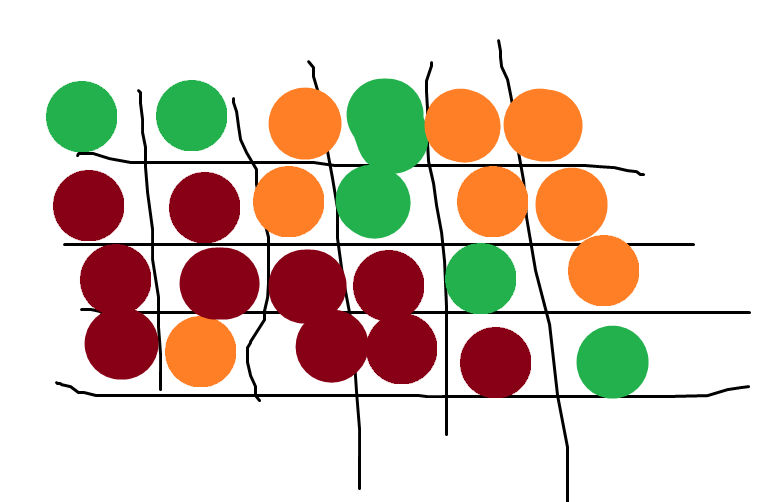
\includegraphics[width=1.\linewidth]{chapters/Results/figures/placeholder_domain_matrix.png}
    \caption{Not done yet}
    \label{fig:PCM-matrix}
\end{figure}

\todo{Find something interesting to discuss}

\section{Parameter Sensitivity Analysis}
No good examination of a model is complete without a Parameter Sensitivity Analysis. That is why I will be making one this week.

% \section{Without gene-defined PCP-initialization}
% \todo{Cut for time or make for appendix}



% \url{https://softmath.seas.harvard.edu/wp-content/uploads/2019/10/2009-07.pdf}
% clear that model is missing cell shape change!
% \section{Additive/subtractive working together matrix}
% \subsubsection{}